\documentclass[tikz,border=10pt]{standalone}
\usepackage{amsmath}
\usetikzlibrary{arrows.meta}
\begin{document}
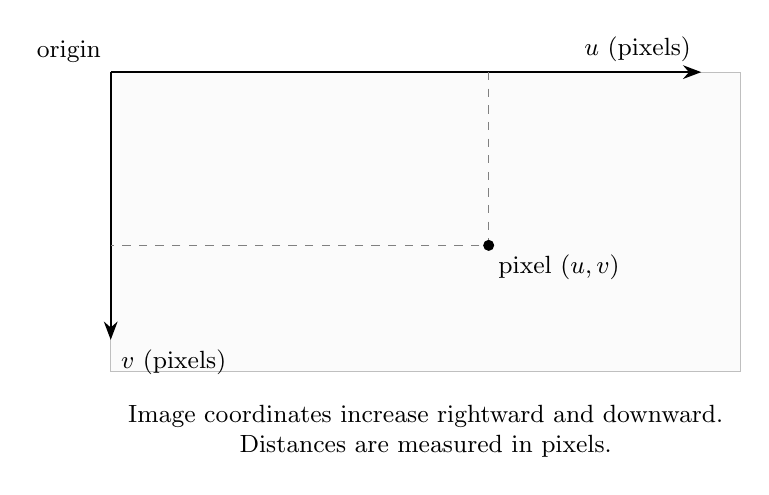
\begin{tikzpicture}[x=1cm,y=-1cm,>=Stealth,font=\small]
\draw[gray!50,fill=gray!3] (0,0) rectangle (8,3.8);
\draw[->,thick] (0,0)--(7.5,0) node[above left] {$u$ (pixels)};
\draw[->,thick] (0,0)--(0,3.4) node[below right] {$v$ (pixels)};
\node[above left] at (0,0) {origin};
\draw[dashed,gray] (4.8,0)--(4.8,2.2)--(0,2.2);
\fill (4.8,2.2) circle (2pt) node[below right] {pixel $(u,v)$};
\node[below,align=center] at (4,4.1) {Image coordinates increase rightward and downward.\\Distances are measured in pixels.};
\end{tikzpicture}
\end{document}
